
\section{Design of AmslerTouch}
In this section, I discuss the design implications and the implementation for the touch-based Amsler grid app: AmslerTouch\footnote{AmslerTouch is a compound word of Amsler+Touch, indicating that the program aims to support with a touch-based, interactive diagnosis.}.

\subsection{Design Implications}

Based on the literature review, I summarized several design decisions for a touch-based, self-reportable Amsler grid application, which are summarized as follows:

\begin{enumerate}
    \item \textbf{The system should offer both (i) fixed-shape tool and (ii) free-shape tool}: In most cases, I identified that the region of symptoms is circular or ellipse, which implies the need for annotating with a circle-shaped tool. Yet, the patient might still want to draw more freely and accurately. Thus, I considered that users should be given a tool for drawing freely as well.
    \item \textbf{The system should offer a color picker for the drawing tool}: As previously noted, AMD is a heterogeneous disease in terms of symptoms, where more than one visual symptoms often appear. Thus, it is reasonable to let users change the color of each markup in order to distinguish each symptom.
    \item \textbf{The system should let users download drawings as an image}: My system ultimately aims to facilitate communication between a patient and medical practitioners. On such an account, it is important for the system to offer a reportable format of drawings.
    \item \textbf{The system should make the user focus on the center of Amsler grid}: As noted in the literature review, it is extremely important to have patients center-align their vision while taking a test. Similarly, I considered it important to induce users to center-align as well in the interface.
    \item \textbf{The system should have users away from a designated distance from the screen}: Since the visual area is relative to the distance from the screen, it is important to keep them away from a fixed distance.
\end{enumerate}

\subsection{AmslerTouch: Web-based Self-reporting Amsler Grid App}

Based on the design implications, I designed AmslerTouch, an interactive web-based Amsler grid app. I discuss some important design elements for inducing successful testing and reporting of symptoms. The overall interface is shown in Figure~\ref{fig:interface}.

\begin{figure}[h!]
    \centering
    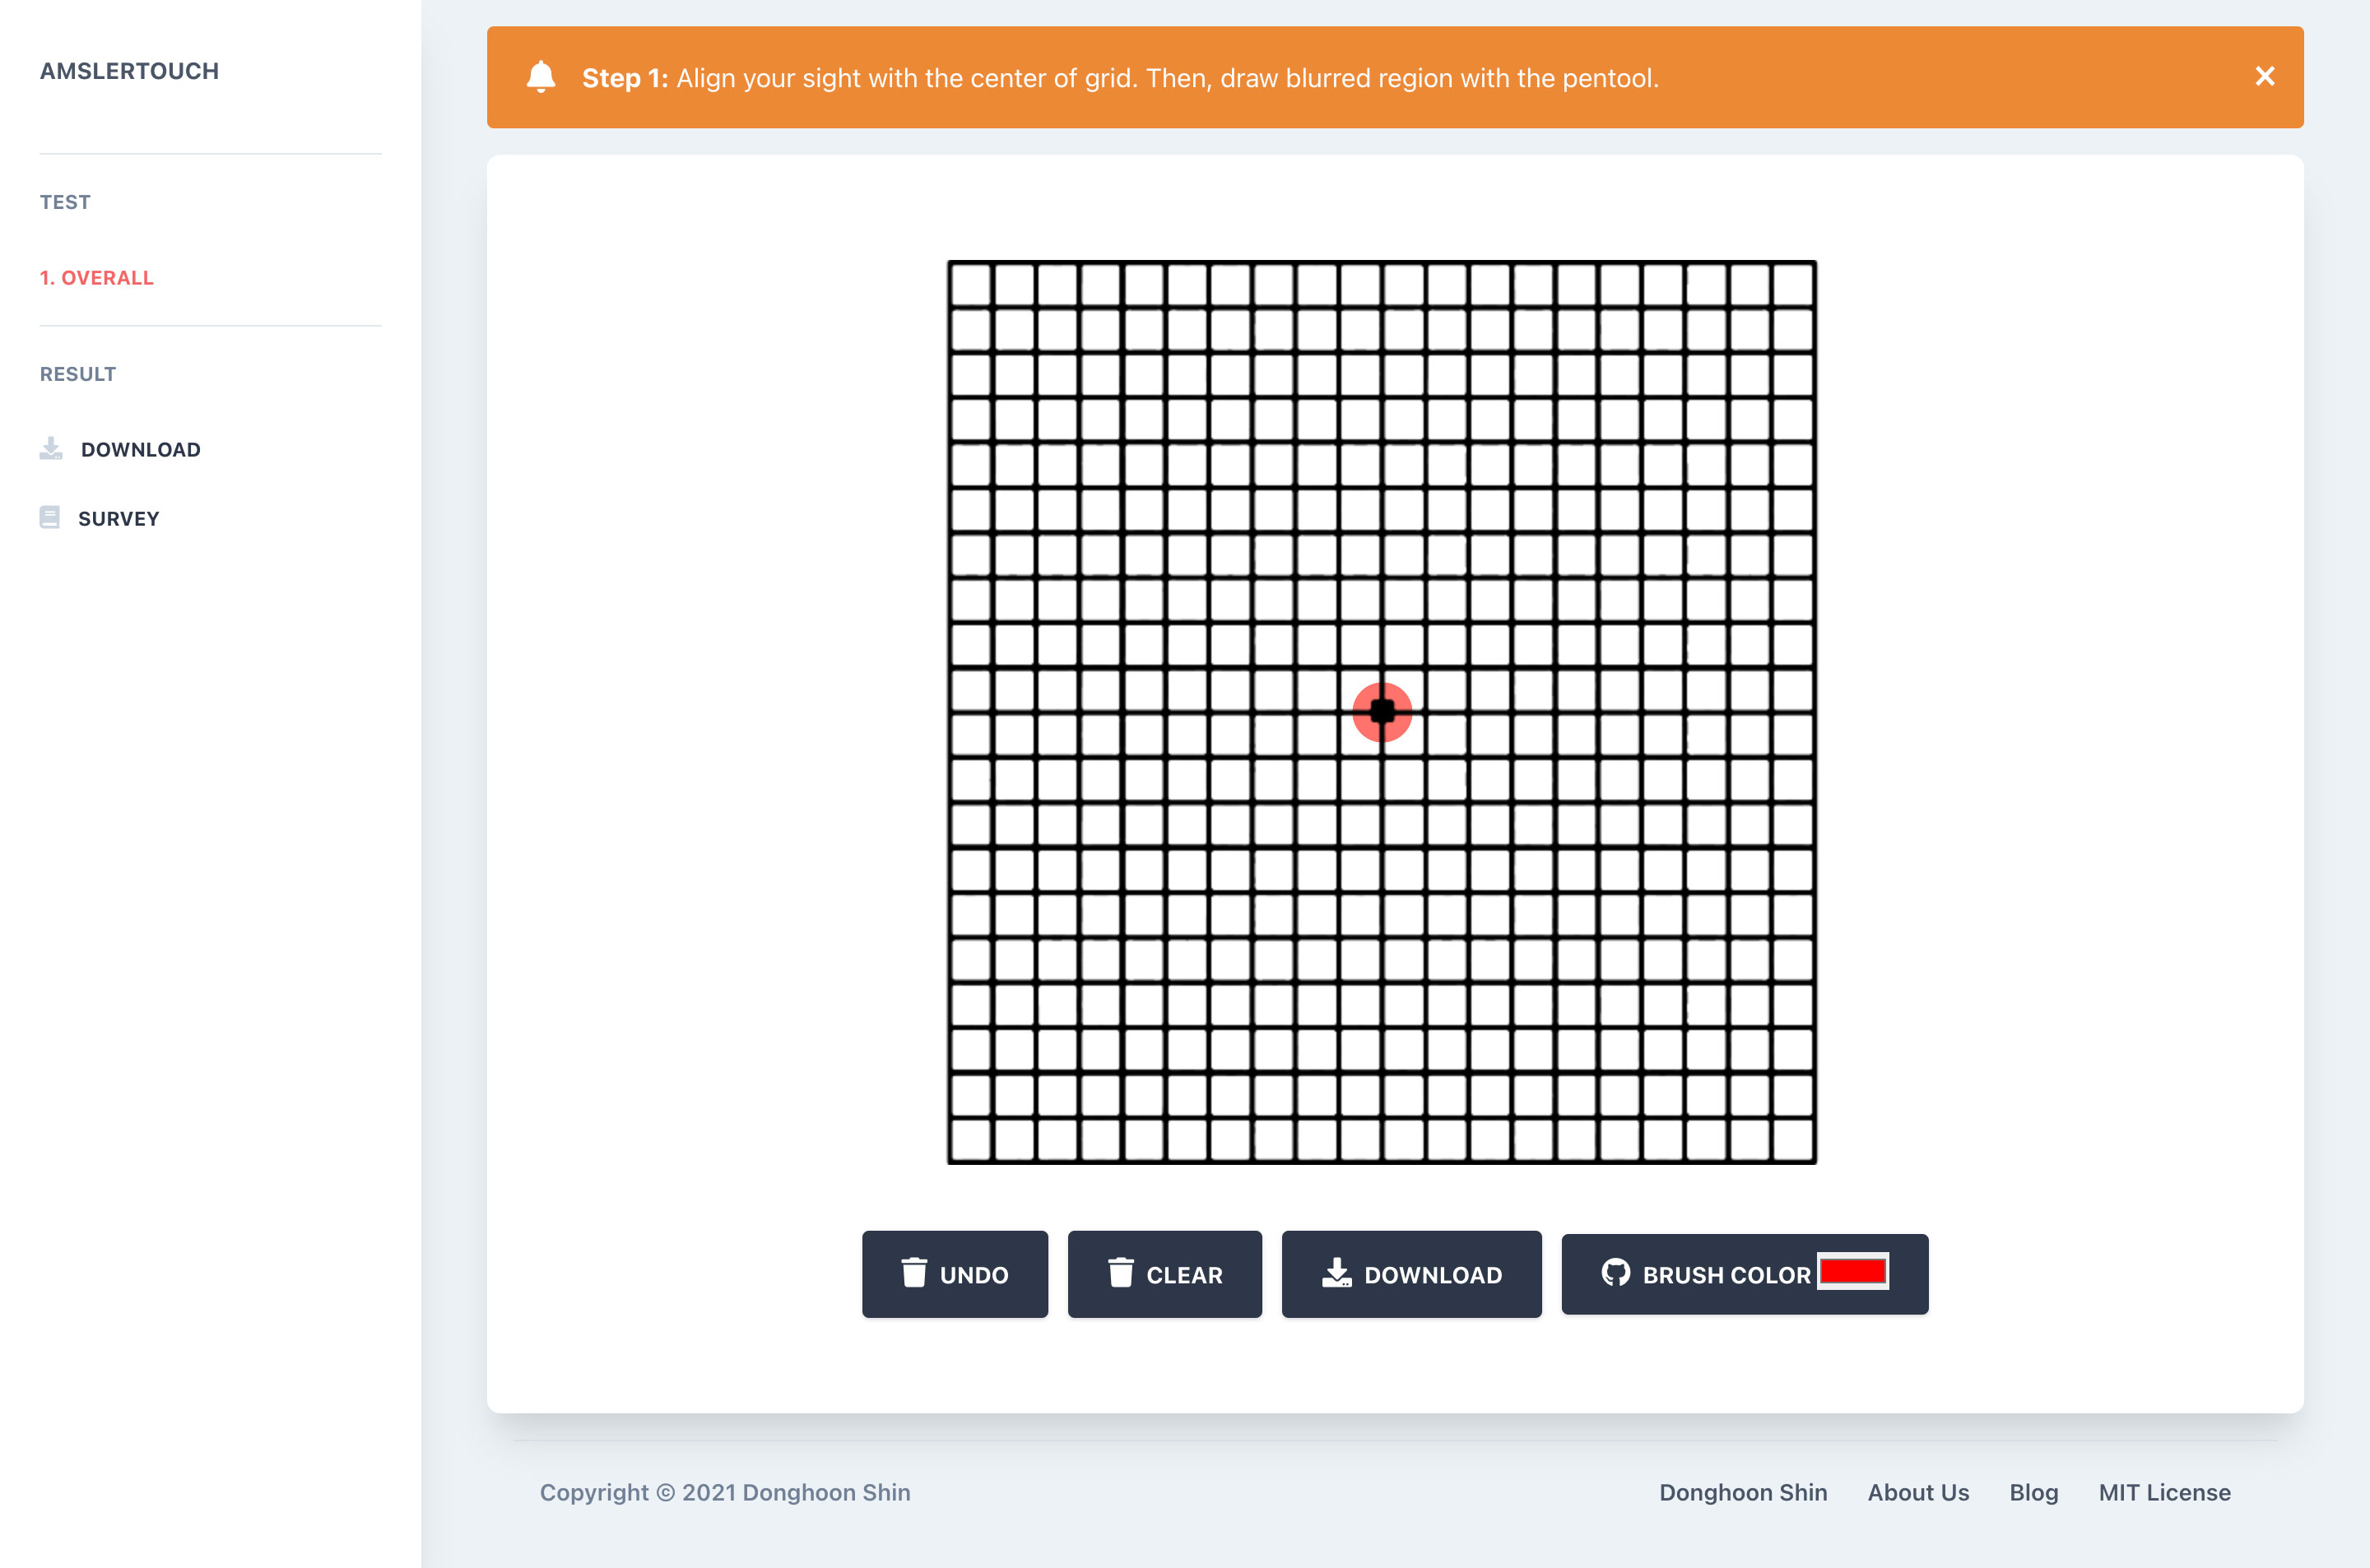
\includegraphics[width=.9\linewidth]{figure/dashboard.jpg}
    \caption{Overall interface of AmslerTouch}
    \label{fig:interface}
\end{figure}

\begin{enumerate}
    \item \textbf{Circle tool and pen tool for drawing}
    
    In order to ensure that users may draw both burden-free and precisely, I applied two types of markup tools for drawing: Circle tool and pen tool. Exemplar usage of each tool is illustrated in Figure~\ref{fig:drawings}.
    
    \textit{(i) Circle tool}. Stemming from the idea that most of the regions of an issue are circular in shape, the circle tool focuses on intuitive use and lets users easily draw. Specifically, once a user presses on a specific region for a long time, a circle is created and enlarged until the user finishes pressing the region.%At the same time, the color filling the circle keeps opaque, making the drawing more intuitive.
    
    \textit{(ii) Pen tool}. Similar to a real-world pencil, pen tool lets users freely draw without any constraint. This tool makes users draw every shape to support precise markup.
    
    
    \begin{figure}[h!]
        \centering
        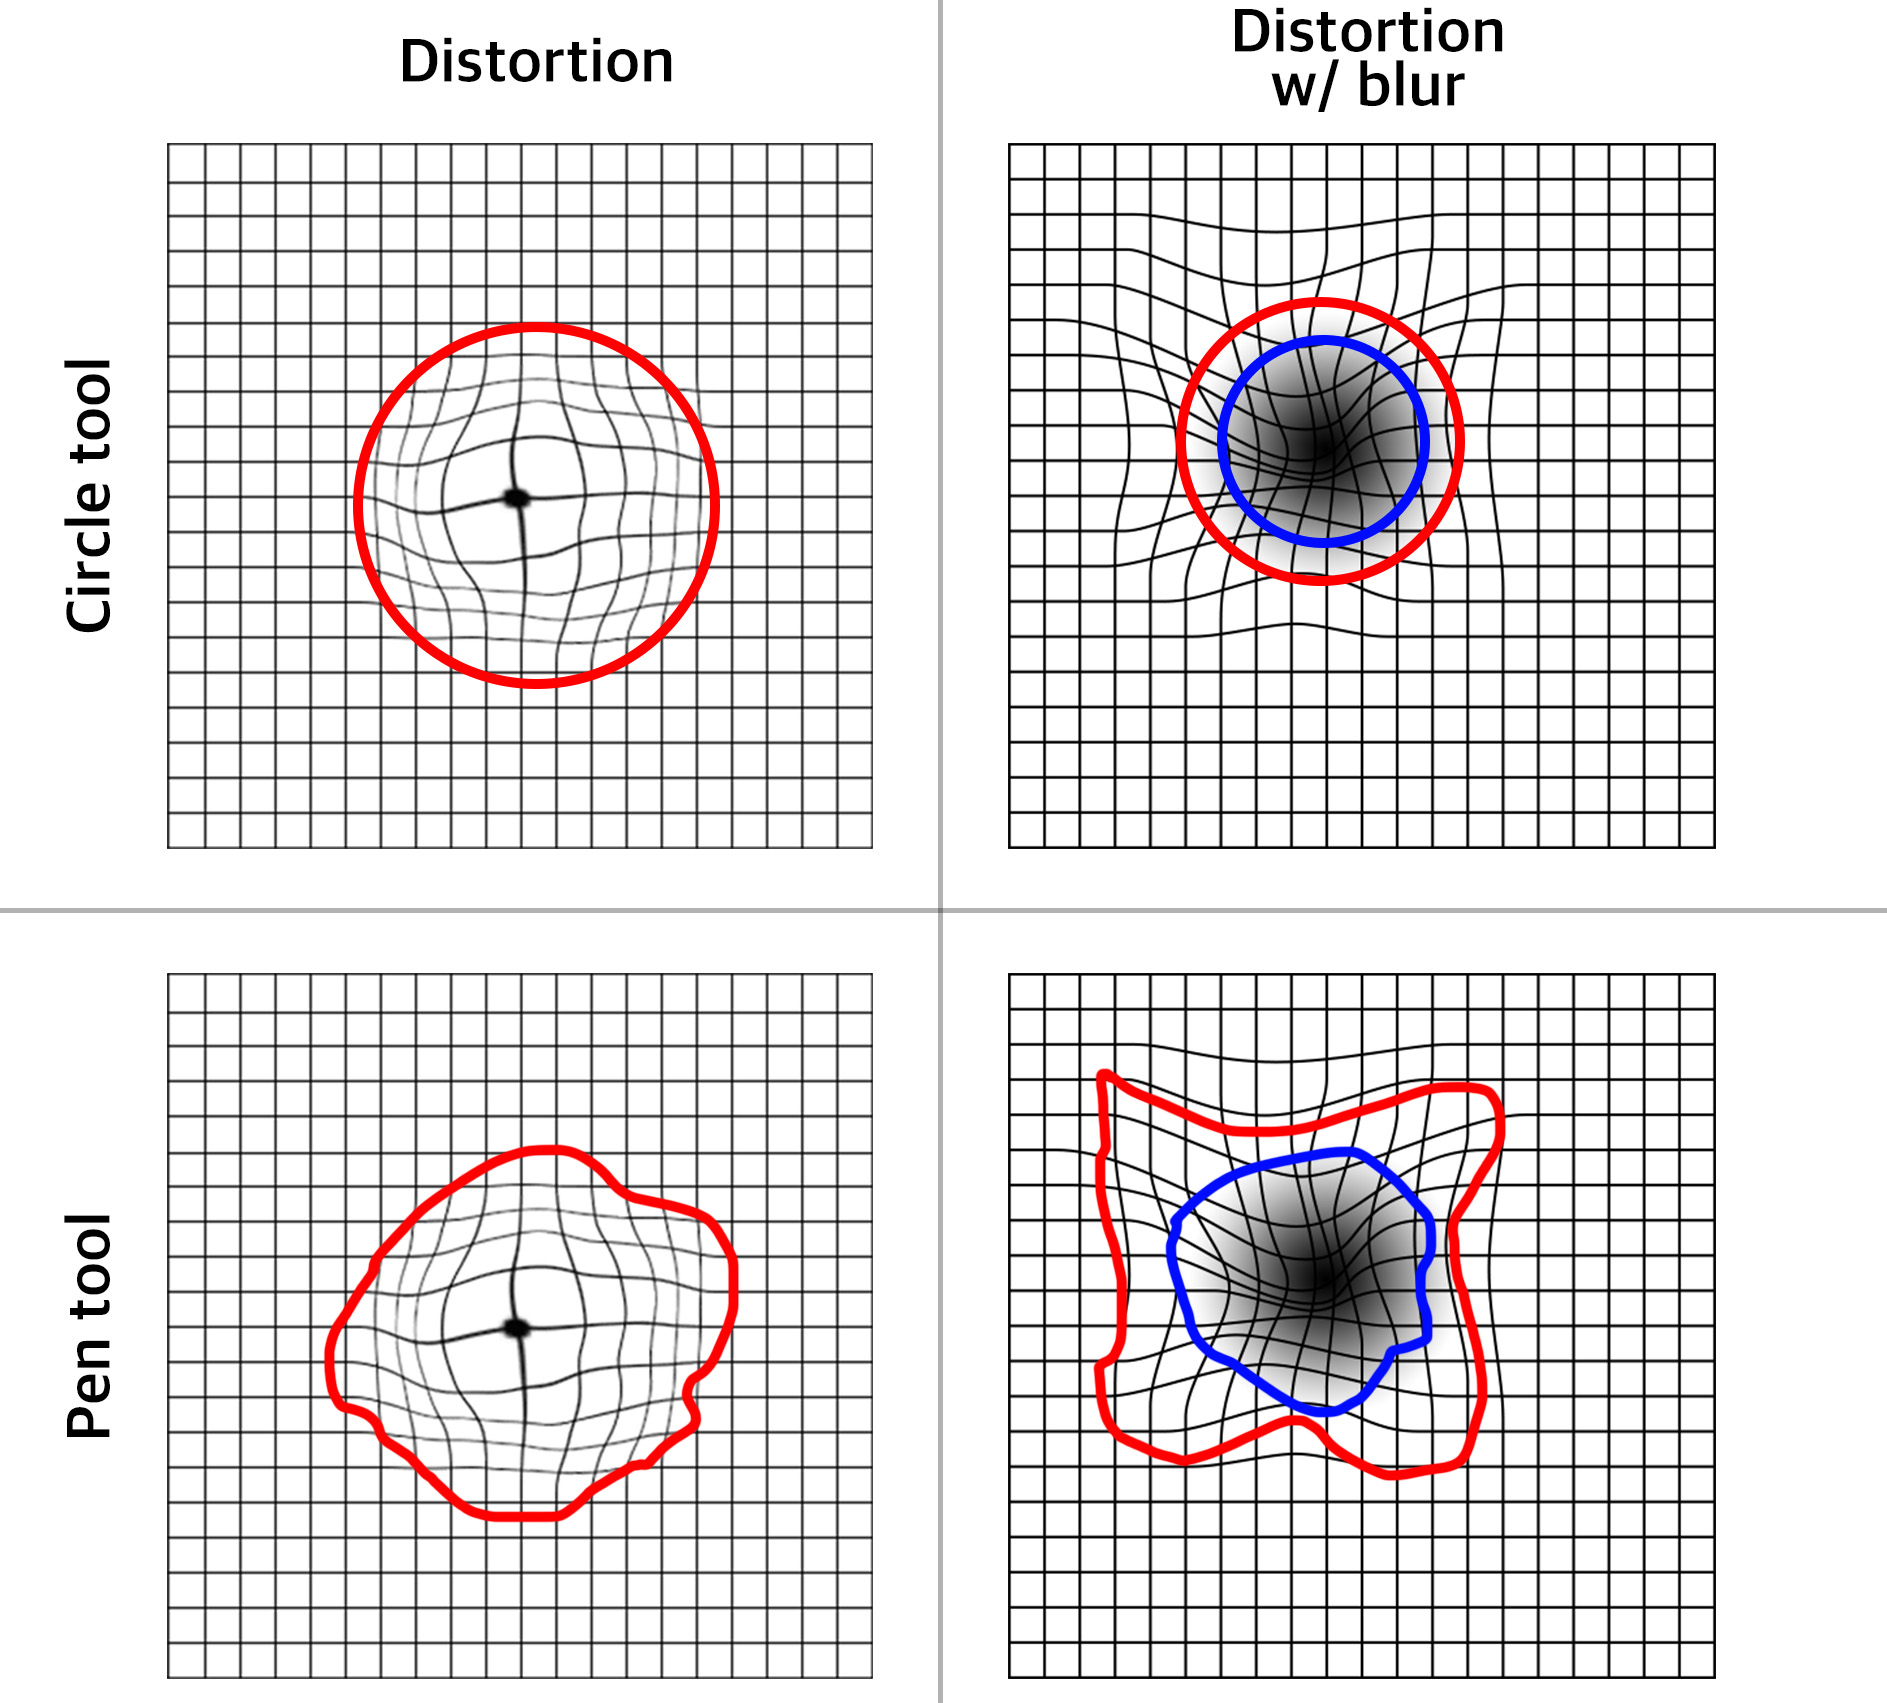
\includegraphics[width=.9\linewidth]{figure/drawings.jpg}
        \caption{An exemplar usage of each tool for each symptom. In this case, red color indicates distortion and blue color indicates blurry region}
        \label{fig:drawings}
    \end{figure}
    
    In order to let users alter their tool easily, I applied an algorithm to change a tool based on the user's initial point of the cursor and point of the cursor after 500ms. To be specific, I considered that if the user moves the position of cursor drastically in 500ms, the user might want to draw using a pen tool. Otherwise, the user is considered to use a circle tool. The algorithm and figure are shown below (Algorithm~\ref{algorithm}, Figure~\ref{fig:distance}).
    
    \newcommand{\factorial}{\ensuremath{\mbox{\sc Factorial}}}
    \begin{algorithm}[h!]
    \begin{algorithmic}[1]
    \Procedure{IsCircle}{$initialPos$}\Comment{Initial position of cursor}
       \State $timer\gets fire$   \Comment{Fire timer}
     \While{$timer.isValid$ and $elapsedTime$ $<$ 500ms}
        \If{$initialPos.distanceTo(currentPos) > 50px$}
        \State{\textbf{return} $false$}
        \EndIf
      \EndWhile\label{euclidendwhile}
      \State{\textbf{return} $true$\Comment{}}
    \EndProcedure
    \end{algorithmic}
    \caption{Determining a suggestion for tool of drawing}
    \label{algorithm}
    \end{algorithm}
    
    \begin{figure}[h!]
        \centering
        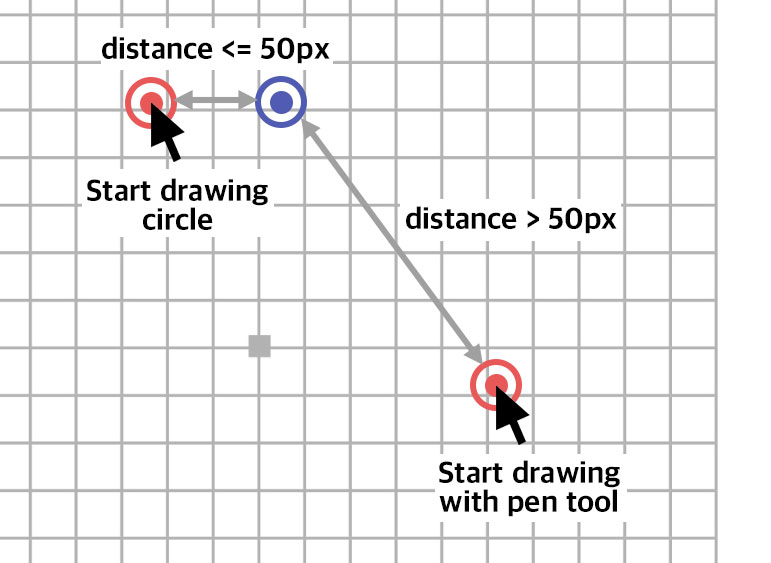
\includegraphics[width=.6\linewidth]{figure/distance.jpg}
        \caption{An algorithm that determines which tool users may want to use. Blue position indicates the initial point}
        \label{fig:distance}
    \end{figure}

    \item \textbf{Color picker for distinguishing markups for different symptoms}
    
    As illustrated in Figure~\ref{fig:colorpicker}, users can choose a color for each drawing to avoid confusion. For example, medical practitioners might ask for a separate drawing for different types of symptoms. In such cases, a single color option for drawings might not be suitable.

    \begin{figure}[h!]
        \centering
        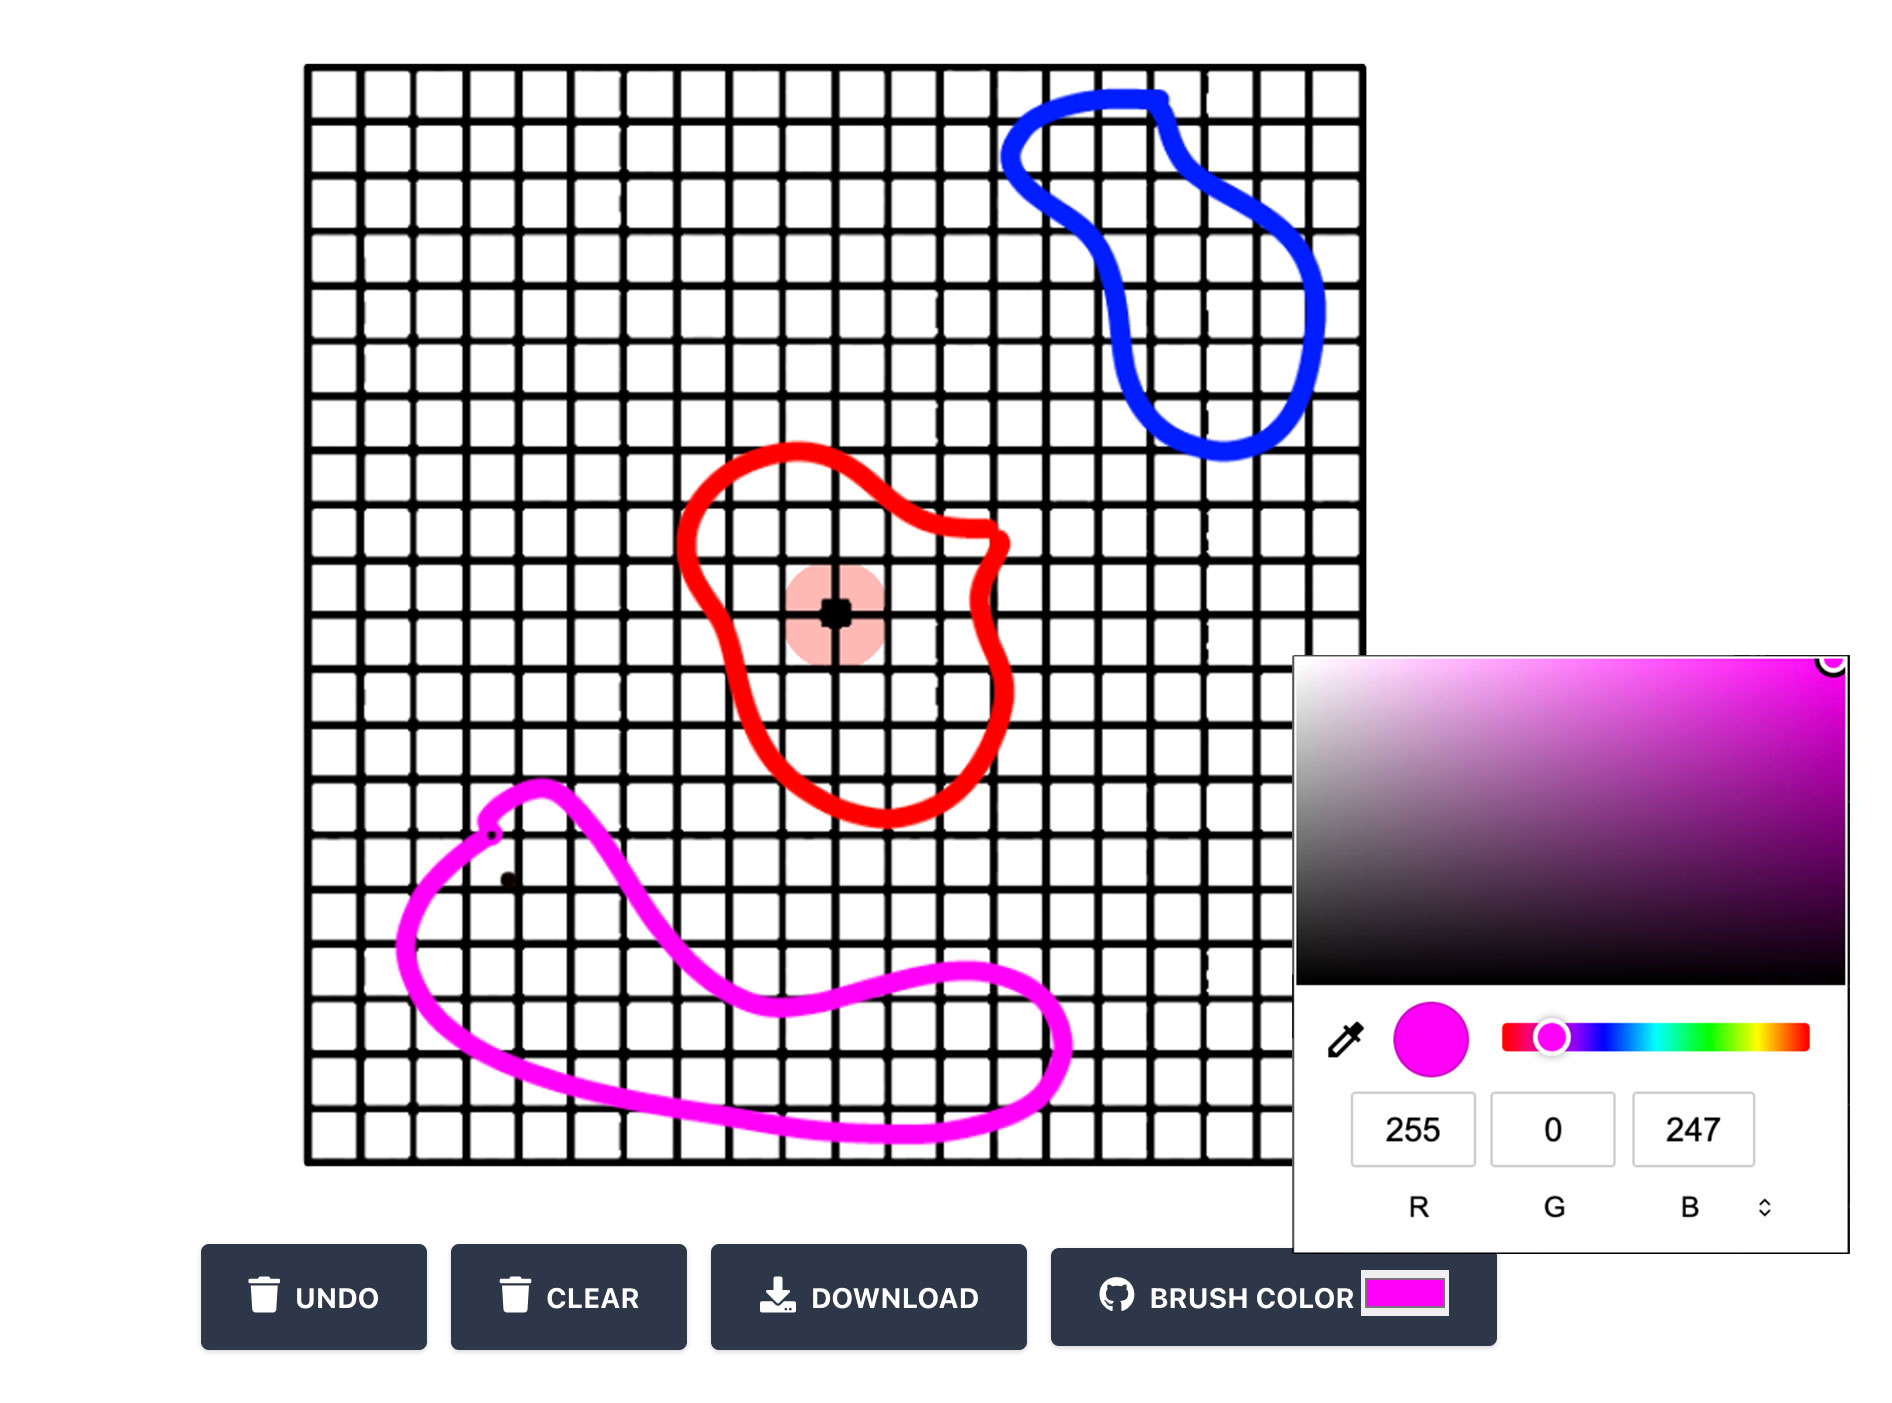
\includegraphics[width=.6\linewidth]{figure/colour.jpg}
        \caption{Color picker for drawings. Users can designate a different color for each drawing}
        \label{fig:colorpicker}
    \end{figure}

    Prior to drawing a new shape, users can choose a new color using the button at the right bottom of the screen. After clicking a color in the palette or designating RGB code, the user can draw with the new color from then.
    
    
    \item \textbf{Download function for saving drawings as an image file}
    
    For medical practitioners to be precisely reported, users should be able to send them imagery. Plus, I considered that medical practitioners and users may easily compare the drawings over time if they are saved as a file. Thus, I added a download function.
    
    \begin{figure}[h!]
        \centering
        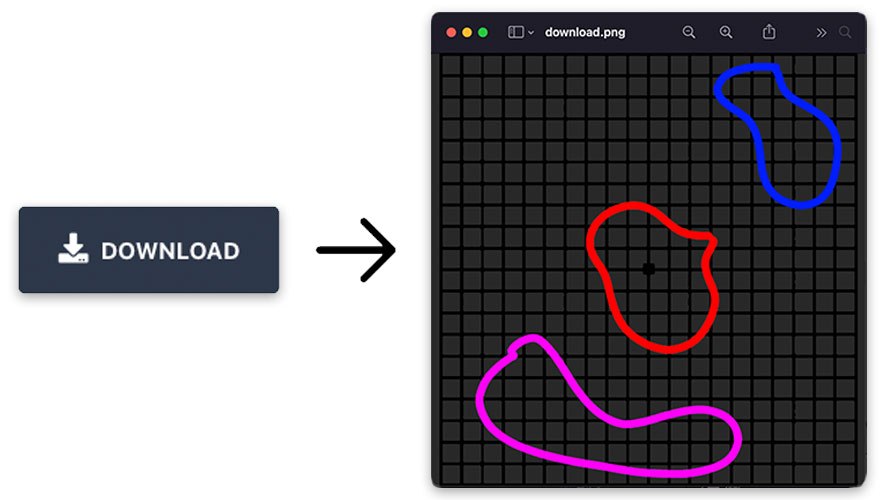
\includegraphics[width=.6\linewidth]{figure/save.jpg}
        \caption{Download function for saving as an image file}
        \label{fig:save}
    \end{figure}
    
    Once the user clicks the download button located at the bottom center (Figure~\ref{fig:save}), the drawings are downloaded as an image (.png). Since the image contains opacity, I considered that the medical practitioners may better understand the scope of the region in a more quantitative way, along with ease of post-processing it.
    
    \item \textbf{A circle-shaped, diffusing animation for inducing users' focus}
    
    It is important to keep the user's vision at the center of Amsler grid while testing. Thus, I designed a spreading circular animation to keep users focused on the center.
    
    \begin{figure}[h!]
        \centering
        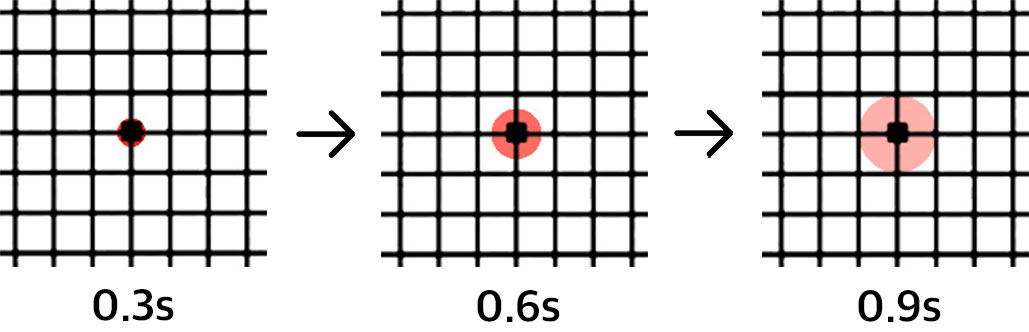
\includegraphics[width=.7\linewidth]{figure/animation.jpg}
        \caption{Center-aligned animation}
        \label{fig:animation}
    \end{figure}
    
    At the center of the grid, a circle keeps growing in size every 1 second (Figure~\ref{fig:animation}). While growing, the opacity of the circle goes down, accordingly making the users perceive as if the circle is diffusing. As such, I aimed to keep users' attention on the center without distracting their sight.

    \item \textbf{A tooltip view for keeping them with a fixed distance}
    
    In order to make users stay away from the screen, I added a tooltip view on top of Amsler grid. As such, I aimed to notice them with how much they should be away from the screen, prior to starting testing.
    
    Amsler grid used for AmslerTouch is 550px * 550px in resolution. Considering that (i) 550px equals 18.6182cm for 75 dpi screen and (ii) 10cm * 10cm Amsler grid testing requires participants to be away from 28 -- 30cm, the system lets users keep 55cm away from the screen. Since the distance decreases as dpi of the monitor goes up, I noted that the figure may vary (Figure~\ref{fig:tooltip}).
    
    \begin{figure}[h!]
        \centering
        
\includegraphics[width=\linewidth]{figure/tooltip.jpg}
        \caption{Tooltip view for inducing users to keep designated distance away from the screen}
        \label{fig:tooltip}
    \end{figure}
\end{enumerate}